\documentclass{article}
\usepackage{graphicx,fancyhdr,amsmath,amssymb,amsthm,subfig,url,hyperref}
\usepackage[margin=1in]{geometry}
\usepackage{xltxtra}
\usepackage{xgreek}
\usepackage{amsfonts}
\usepackage{amssymb}
\usepackage{amsmath}
\usepackage{amsthm}
\usepackage{mathtools}
\usepackage{tabu}
\usepackage{caption}
\usepackage{ subfig}
\setmainfont[Mapping=tex-text]{Times New Roman}
%----------------------- Macros and Definitions --------------------------

%% FILL THIS OUT
\newcommand{\studentname}{Νικόλαος Ζαρίφης}
\newcommand{\suid}{03112178}
%% END



\renewcommand{\theenumi}{\bf \Alph{enumi}}

%\theoremstyle{plain}
%\newtheorem{theorem}{Theorem}
%\newtheorem{lemma}[theorem]{Lemma}

\fancypagestyle{plain}{}
\pagestyle{fancy}
\fancyhf{}
\fancyhead[RO,LE]{\bfseries\large NTUAthens}
\fancyhead[LO,RE]{\bfseries\large Λάμδα Λογισμός}
\fancyfoot[LO,RE]{\bfseries\large \studentname: nick.zarifis@hotmail.com}
\fancyfoot[RO,LE]{\bfseries\thepage}
\renewcommand{\headrulewidth}{1pt}
\renewcommand{\footrulewidth}{1pt}

\graphicspath{{figures/}}
\usepackage{tikz}
%-------------------------------- Title ----------------------------------

\title{Category Theory \\}
\author{\studentname \qquad  ID: \suid}

%--------------------------------- Text ----------------------------------
\DeclarePairedDelimiter\floor{\lfloor}{\rfloor}
\newtheorem{lemma}{Lemma}
\begin{document}
\maketitle
\section*{Βασικοί ορισμοί}

Η θεωρία κατηγορίας έχει να κάνει με μορφισμούς συναρτησεων ,όπως στην ανάλυση που έχουμε διαφόρες συναρτήσεις έτσι έχουμε κι εδώ το ίδιο πράγμα αλλά πιο γενικευμένα δηλάδη δεν χρειάζεται να κάνει map σε αριθμούς ή απο αριθμούς σε αριθμούς, αλλά γενικά από ότιδηποτε σε ότιδηποτε. Συνήθως της συναρτήσεις τις αποκαλούμε και μορφισμούς.

\large {Κατηγορία:}
\begin{itemize}
	\item  Περιέχει ένα σύνολο απο αντικείμενα. Συμβολίζεται ως obj(C).
	\item Ένα σύνολο απο μορφισμούς. Βλέπτε $f:a\rightarrow b$ κι το συμβολίζουμε ως$hom_C(a,b)$ , το σύνολο των μορφισμών τις κατηγορίας C απο το α στο β.
	\item Περιέχει την δυαδική πράξη της σύνθεσεις μορφισμών. Συμβολίζω με dot(.) . Και η πράξει περιέχει τα αξιώματα της προσετεριστικότητας κι της υπαρξείς ουδέτερου στοιχείου (Συμβολίζουμε με $id_A : A\rightarrow A$). 
	\end{itemize}
Επίσεις μπορούμε να όρισουμε μεταξύ 2 κατηγορίων μια συνάρτηση όπου θα αντιστοιχεί αντικείμενα απο την μια κατηγορίας στην άλλη,Αυτές τις συναρτήσεις τις αποκαλούμε Functors. 
Δηλάδη έστω ότι έχουμε έναν functor $F: C_A \rightarrow C_B$ τότε αν έχουμε $a \in obj(A) \rightarrow F(a)\in obj(B)$ .
\\Επίσεις τον επεκτήνουμε στις συναρτήσεις κι στην σύνθεση ως: \\
Έστω συνάρτηση $f: a_A \rightarrow b_A$ τότε η $F(f):F(a_A)\rightarrow F(b_A)$.\\
Στην σύνθεση $F(f.g)=F(f).F(g)$ και φυσικά ως προς το ουδέτερο στοιχείο.
$F(id_A)=id_{F(A)}$.\\
Θα ήταν λάθος μου να μην αναφαίρω τις δυνατότητες που έχουν οι functors στον προγραμμάτισμο κι στον λάμδα λογισμό. Κατάρχας αυτό που θα δείξουμε αργότερα είναι ότι οι Καρτεσιανές Κλείστες Κατηγορίες (βλ. παρακάτω) μπορούμε να τις μετατρέψουμε σε όρους λαμδα-λογισμού με απλούς τύπους. 
Όταν δουλεύουμε σε ένα προγραμμά μπορούμε να σκεφτούμε την κατηγορίας ως ένα κυβώτιο που περιέχει κάποιον τύπον πχ λίστες, δέντρα κτλπ. Ας πούμε λοιπόν ότι έχουμε όρισει ένα σύνολο συναρτήσεων πάνω σε έναν τύπο κι στην συνέχεια θέλουμε να το εφαρμόσουμε σε ένα κυβωτίο τύπων χωρίς όμως να ξαναόρισουμε κάθε συναρτήση ξανά. Απλά να σκεφτούμε ότι σε ένα προγραμμά με εκατοντάδες συναρτήσεις κάτι τέτοιο θα ήταν χρονόβορο. Έτσι λοιπόν μπορούμε απλά να φτιάξουμε έναν functor που να αντιστοιχεί στο κάθε ίδους κυβώτιο πχ ένα παράδειγμα στην  haskell που έχουμε high order functions έστω ότι έχουμε όριση την πολύ απλή συνάρτηση:
\\add5: Int->Int
\\add5 x = x+5  \\
Κι έχουμε έναν σύνθετο τύπο δέντρο όπως:\\
data Int tree = Leaf of Int | Node of Int * tree *tree 

Για να έφαρμόσουμε την add5 σε όλα τα στοιχεία του δέντρου απλά όριζουμε έναν Functor γιαυτή την δουλιά .
\\myfunctor : (Int->Int)->(Int tree->Int tree)
\\myfunctor id  tree =id tree
\\myfunctor f (Leaf a) = f(a) 
\\myfunctor f (Node a,left,right) = Node (f a, myfunctor f left,myfunctor f right)

Έτσι λοίπον μπορούμε να όρισουμέ την \\ add5tree = myfunctor add5 
κι γλιτώσαμε αρκετό κόπο.
Την ένοια του functor πολλές γλώσσες προγραμματισμού την ύποστηρίζουν πέρα απο συναρτησιακές αλλά και Αντικειμενοστραφείς και μερικές προστακτικές .
\\
Επίστρεφοντάς 2 ακόμα συμαντικόυς όρισμούς: \\
\begin{itemize}
 	\item [\textbf{Intial Object}] Είναι υπάρχει έναν αντικείμενο που οι μόνοι μορφισμοί που υπάρχουν είναι απο αυτό σε όλα τα άλλα αντικείμενα.
	\item [\textbf{Terminal Object}] Είναι το δυικό δηλαδή όταν υπάρχει έναν αντικείμενο που οι μόνοι μορφισμοί που υπάρχουν είναι απο  όλα τα άλλα αντικείμενα σε αυτό .
\end{itemize}
\large {\textbf{Δυική Κατηγορία:}}\\
Μπορούμε σε μια κατηγορία να όρισουμε την δυική της κατηγορία η οποία είναι με τα ίδια αντικείμενα αλλά με ανεστραμένους τους μορφισμούς. Όπως είανι κι προφανές η σύνθεση αλλάζει δηλάδη αν είχα την $G=f.g$ τώρα θα έχς την $G^{-1}=g^{-1}.f^{-1}$ .Αυτή η σχέση μας θυμίζει στους δυανισματικούς χώρους όταν έχω έναν πίνακες τάξης n ισχυεί ακριβώς ο ίδιος τύπος αντιστροφης άρα μπορούμε να βρούμε δυανισματικούς χώρους που είναι κατηγορίες. Φυσικά στην δυική κάθε terminal γίνεται initial κι αντίστροφα.

\large{\textbf{Products}} \\
Θα λέμε ότι ένα αντικείμενο είναι product (γινόμενο) 2 αντικείμενον ανν όριζουμε 2 μορφιφούς προβολών του Χ, έστω $X=X_1*X_2$\begin{itemize}
	\item $\pi_1 : X\rightarrow X_1$ 
	\item $\pi_2 : X\rightarrow X_12$ 
	\end{itemize}
Και επίσεις έστω οι μορφισμοί $f: Y\rightarrow X$ και $f_1: Y\rightarrow X_1$ , $f_2: Y\rightarrow X_2$ έτσι ώστε: $f(Y)= f_1(Y)*f_2(Y)$. Κι σε σχήμα:
\\ 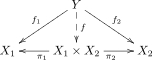
\includegraphics[height=100pt,width=100pt]{product.png}

\large {\textbf{Expomential object}}\\
Αν έχουμε 2 αντικείμενα στην κατήγορία όριζουμε ως $X^Y$ το σύνολο των μορφισμων απο το Υ, Χ . 
\\Κι θα ορίσουμε με την σείρα μας 2 πολή συμαντικές συναρτήσεις:
\\Την eval $eval_{A,B}: B^A * A \rightarrow B$ . Όπως φαίνεται κι απο τον τύπο 
ισχυεί ότι $eval_{A,B}(f,A)=f(A)$.
\\ Και την curry έτσι ωστε αν έχουμε έναν μορφισμό g τότε $curry_c(g) : C\rightarrow B^A$ και ισχυεί οι $eval_{A,B}.(curry_c(g)*id_A)=g$ . 

\section*{Cartesian Closed Categories -CCC}

Μια κατηγορία λέγεται Καρτεσιανή κληστή αν:
\begin{itemize}
	\item Έχει terminal object. (Έστω 1)
 	\item Για κάθε 2 αντικείμενα έχουμε μέσα στην κατηγορία κι το γινόμενο τους.
	\item Για κάθε 2 αντικείμενα έχουμε κι το $X^Y$. 
	\end{itemize}
Η κατηγορία των συνόλων που έχει ως αντικείμενα τα σύνολα κι της συναρτήσεις ως μορφισμούς, είναι CCC.Αυτή την κατηγορία θα χρησιμοποιούμε απο έδω κι παρακάτω γιατί θα αναθέσουμε τους τύπους του λάμδα λογισμού σε σύνολα. 
 
\section*{Categorial Model for simply-typed lamda-calculus}

Αν λοιπόν θεωρήσουμε τα αντικείμενα ως τύπους κι τους όρους ως μορφισμούς , μπορούμε να όρισουμε μια δομή πάνω στος CCC.

Όριζουμε μια δομή Μ πάνω στην CCC $C$ (υποθέτουμε ότι η κατηγορία είναι πάνω σε set φυσικών αριθμών) για τον λαμδα λογισμών απλών τύπων (μαζί με το γινόμενο τύπων) ως:\\
\begin{itemize}
	\item	Ορίζουμε το τερματικό στοιχείο (συμβ. 1) να έχει τύπο nil (void,() κτλπ) ο μοναδιαίος τύπος 
	\item Όριζουμε μια συνάρτηση F ως έξείς: \\
		Για κάθε αρχικό τύπο t F(t) είναι ένα αντικείμενο.\\
		Για $F(t\rightarrow t_1) = F(t)^{F(t_1)} $\\
		Για $F(t*t_1) = F(t)*F(t_1) $
	\item Έστω $H= x_1 :t_1 \dots \dots ,x_n:t_n$ τότε:\\
		$F()=1$\\
		$F(x:t)=1*F(t)$\\
		$F(H)=F(x_1:t_1 \dots\dots,x_{n-1}:t_{n-1})*F(t_n)$
\item Αν $H \vdash M:t$ τότε $F(H \vdash M:t): F(H) \rightarrow F(t)$.
\item 
	Υπάρχει σημείο $F(c):1 \rightarrow F(\Sigma)$. Που το $\Sigma$ είναι όλοι οι απλοί τύποι.
Απο τον ορισμό καταλαβαίνουμε πως η F είναι μια συναρτησή αποτίμησης. Έτσι ερμηνεύουμε ιδιότητες τις CCC στην simple typed lambda calculus.
\end{itemize}
Έτσι λοιπόν η ερμηνεία επεκτήνεται στους όρους ως:
\begin{itemize}
	\item $F(H \vdash c:t) =F(c).t_A$όπου $t_A$ είναι ο μορφισμός από το Α στο τελικό στοιχίο 1 (Nil).
	\item $F(H \vdash x_i : t_i)=\pi_i$
	\item Στην αφαίρεση: $F(H \vdash \ \lambda x : u . N \: u => v)$ =$ curry(F(H , x : u \vdash N : v))$
	\item Εφαρμογή: $F(H \vdash LN:s) = eval . <F(H\vdash L: t=>s),F(H \vdash N:t)>$
	\item Ζευγή $F(H \vdash (L,N): s*t)=<F(H\vdash L:s),F(H \vdash N:t)>>$
	\item first $F(H \vdash fst(N):s)=fst . F(H \vdash N : s*t)$
	\item second $F(H \vdash snd(N):s)=snd . F(H \vdash N : s*t)$
\end{itemize}

\textbf{Ορισμός:} Έχοντας μια δομή S σε μια CCC έστω C αν έχουμε την εξίσωση $H \vdash M_1 = M_2 :t$ τότε λέμε ότι το S ικανοποιεί την εξίσωση αν $F(H \vdash M_1:t)$ και  $F(H \vdash M_2 :t)$ είναι οι ίδιοι μορφισμοι στο C.
Και το γράφουμε ως: \\
$S \models H \vdash M_1 = M_2 :t$.\\
Και λέμε ότι το  S είναι μοντέλο της simple typed lamda calculus θεωρίας $T = (\Sigma,Ax)$ αν το S ικανοποιεί όλες τις εξισώσεις στο Ax δηλαδή $S \models Ax$.

Κι αποδυκνείωντας ότι όλοι οι κανόνες του lamda λογισμού είναι sound στο μοντέλο που κατασκευάσαμε, καταλήγουμε στο πολύ συμαντικό συμπέρασμα:

\textbf{Soundness for CCC-Models} \\
Αν C είναι μια CCC και $T=(\Sigma,Ax)$ και S ένα μοντέλο της Τ στο C αν $T \vdash (H \vdash M=N:t)$ τότε $S \models H \vdash M=N:t$
\\ Για να το αποδείξουμε , δείχνουμε την ορθότητα της α-ισοδυναμίας, τις η-ισοδυναμιας κι της β-αναγωγής.\\
Ως παραδείγμα θα δείξουμε την ορθότητα της β-αναγογης.\\

\begin{proof} 
Έστω\\ $H \vdash \lambda x :s.M :s=>t$  και $H \vdash N:s$\\ τότε έχουμε:\\ $F(H \vdash (\lambda x :s.M)(N):t)$\\$=eval.<F(H \vdash \lambda x : s.M s=>t),F(H \vdash N:s)> $ \\$= eval.<curry(F(H,x:s \vdash M:t)),F(H \vdash N:s)>$\\
Στην CCC έχουμε ότι\\ $(f*h) . <g,k> = <f.g,h.k>$ και $<g,k>=<g*id>,<id,k>$.\\
και έχουμε:\\ $L.H.S.= eval. curry(F(H,x:s \vdash M:t)*id_{F(s)}).<id_A,F(H \vdash N:s) > =F(H,x:s \vdash M:t) .<id_A,F(H \vdash N:s)> = F(H\vdash [N/x]M:t)$
\\Η τελευταία ισότητα ισχυεί απο λήμμα αντικατάστασεις, που εδώ το ορίζουμε ως: \\Αν $f =F(H,x:s\vdash M:t):A*B \rightarrow C$ και $g=F(H \vdash N:s)A\rightarrow B$ .Τότε $F(H \vdash [N/x]M:t)=f.<id_A,g> :A \rightarrow C$ 
\end{proof} \\
 \textbf{Completness }
 \\
       Αν  $H \vdash M:a$ και $H \vdash N:a $ τότε υπάρχει μια CCC (F) έτσι ώστε αν :  $F(H \vdash M:a)=F(H \vdash N:a)$ τότε $H \vdash M = N :a$ .
 \\  \\
\section*{Curry-Howard-Lambek correspondence}
Τελειώνοντας Θα δούμε κι τι γίνεται με τον ισομορφισμό Curry-Howard–Lambekc . 
Το 1970 ο Lambek έδειξε ότι οι αποδήξεις στην ιντουζιανή λογική , typed lambda calculus και στις CCC με αντικείμεντα ως τύπους κι μορφισμούς ως όρους κι αποδείξεις.Επεκτήνοντας δηλαδή τον CH isomorphism που είδαμε στο μάθημα.
\\
Δηλαδή:\\ Κάθε απόδειξη είναι μια παραγωγή τύπων. \\
Κάθε παραγωγή τύπων ισοδυναμεί με έναν καλά ορισμένο λάμδα όρο.\\
Άρα:Αποδείξεις θεωρημάτων κωδικοποιούνται ως κλειστεί τύποι και οι υποθέσεις κωδικοποιούνται απο το περιβάλων του τύποθ.
Αναλητικά έχουμε ότι:
ορίζουμε ως nil το τελικό object .
Θεωρούμε λοιπόν κάθε μορφισμό απο τον τύπο a στον τύπο b δηλαδή $f: a \rightarrow b$ ως , αν το θεωρημά a ισχυεί τότε ισχυεί κι το θεώρημα b.
Καταρχάς μετασχηματίζουμε έτσι ωστέ να θεωρούμε τα products ως and δηλαδή $a*b= a \land b$
Κρατάμε εδώ τους μορφισμούς που έχουμε όρισει, δηλαδή τους id,curry,eval και προβολές .
\\Ο id δείχνει την αποδείξη:\\ $id: a\vdash a$ . \\
Η σύνθεση μορφισμών:\\
\begin{tabular}{l  c}
	$f: a\vdash b$ & $g: b \vdash c$
\\	\hline
	$f.g : a \vdash c$
\end{tabular}
\\  Unit:\\
\begin{tabular}\\
 \hline
$ \star : a \vdash Void$\\
\end{tabular}
\\
Cartesian Product:\\
\begin{tabular} {l c}
	$f: a\vdash b$ & $g: a \vdash c$
\\	\hline
	$f*g : a \vdash b*c$\\
\end{tabular}
\\Προβολές:\\
\begin{tabular}
\\	\hline
	$\pi _1 : a*b \vdash a$
	\\
	
\\	\hline
	$\pi _2 : a*b \vdash b$ \\
\end{tabular}
\\Curry:\\
\begin{tabular}
	$f : a*b \vdash c$ 
\\	\hline
	$curry\ f : a \vdash b \rightarrow c$
\end{tabular}
\\Εφαρμογή:\\

\begin{tabular}
\\	\hline
$eval: (a\rightarrow b ) *a \vdash b$\\
\end{tabular}\\
Έτσι λοιπόν έχουμε ότι υπάρχει μορφισμός f έτσι ώστε $f: a_1 *a_2*\dots a_3 \vdash b$ ανν to $a_1,a_2,\dots ,a_n \vdash b$ στην ιοντουζιανή λογική.
\\
\begin{theorem}
	Η $\lambda$ -Calculus κι οι CCC είναι ισομορφικές.Συγκεκριμένα CL$\cong$ id και LC $\cong$ id.
\end{theorem}
Όπου C ένας functor απο την Lambda Calculus στην CCC, κι  L το αντίστροφο
\section*{Αποτελέσματα CHL correspondance:}
\begin{itemize}
\item {Λογική: υπολογιστίκο περιεχόμενο αποδίξεων }
\item {CS: Θεμέλεια type-system και συναρτησιακού προγραμματισμού. Αν σκεφτούμε ότι η Haskell βασίζεται στην  Category Theory}
\item {Category Theory:Μια σύνδεση στις γλώσσες κι στην λογική.
\\
Λαμβδα λογισμός ως γλώσσα για τις CCC.
Λαμδα λογισμός για υπολογισμούς σε θέματα περί CCC και αντιστρόφος.}
\item{Monads : Είναι μια δομή πάνω σε μια κατήγορία απο την οποία μπορούμε να παράγουμε υπολογιστή μοντέλα, κι ντετερμινιστικά που είναι ισοδύναμα με την μηχανή turing και μη ντετερμινιστικα , ένα καλό παράδιγμα μη ντετερμινιστικού μοντέλου είναι ο List Monad της γλώσσας Haskell} 
\end{itemize}
\section*{Βιβλιογραφία:}
\begin{itemize}
	\item Curry-Howard-Lambek Correspondence by Subashis Chakraborty
	\item Category Theory and the Simply Typed $\lambda$-Calculus by Alfo Martini
		\end{document}
